\subsection{Radiolichtkurve der Sonne}

Für die gemessene Flussdichte des Teleskops gilt
\begin{equation}
S(\nu) = \frac{2 \, k_B \, T_{Ant}(\nu)}{A_{eff}}. 
\end{equation}

Durch Umstellen nach $A_{eff}$ ergibt sich: 

\begin{equation}
A_{eff} = \frac{2 \cdot \, k_B \, T_{Ant}(\nu)}{S(\nu)} = \frac{2 \cdot \, 1.38 \cdot 10^{-23} \frac{J}{K} \, 35000 K}{170.3 \, \mr{sfu}}\approx 56.7\  m^2.
\end{equation}
Da das Teleskop etwa kreisförmig mit einem Radius von 2.3 m ist, ergibt sich eine effektive Fläche von etwa 16.6 $m^2$. \\
Da das Maximum der Strahlung ergibt sich deshalb zu $5.8 \cdot 10^{-20} \frac{W}{Hz \, m^2}$.
Die effektive Fläche liegt also in der gleichen Größenordnung, wie die tatsächliche Fläche. Die Differenz ist durch die erhöhte Sonnenaktivität und die zu hohe Kalibrierungstemperatur zu erklären. Normale Werte lägen bei $T_\mathrm{Ant}\approx 250\,K$ und $S(0)=95\,\mr{sfu} $. Damit erg"abe sich ein Wert von 0.73 $\mr{m}^2$. Die effektive Fl"ache ist somit weitaus kleiner als die tats"achliche Fl"ache.

%\begin{figure}
%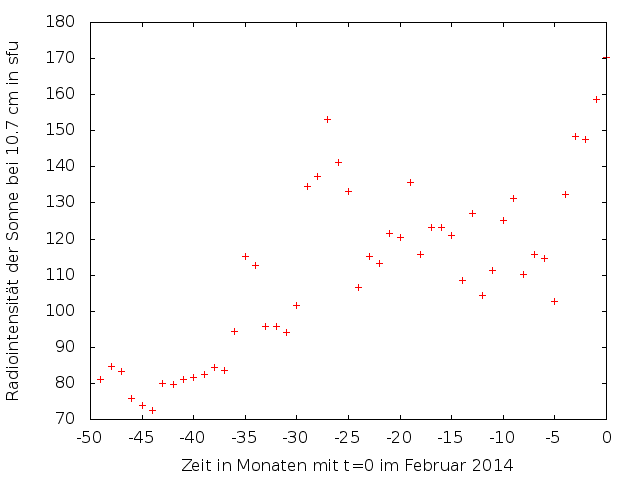
\includegraphics[width=.8\textwidth]{images/sun3.png}
%\caption{Radiolichkurve der Sonne}
%\label{fig:radiokurve}
%\end{figure}

%\begin{figure}
%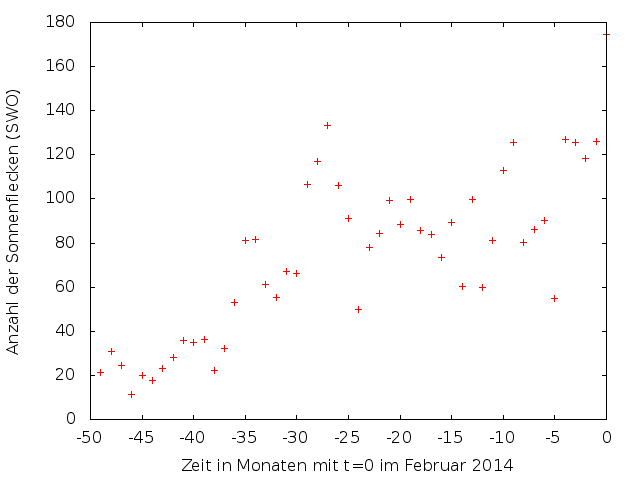
\includegraphics[width=.8\textwidth]{images/sun4.png}
%\caption{Anzahl der Sonnenflecken der Sonne}
%\label{fig:radiokurveflecken}
%\end{figure}

\begin{figure}
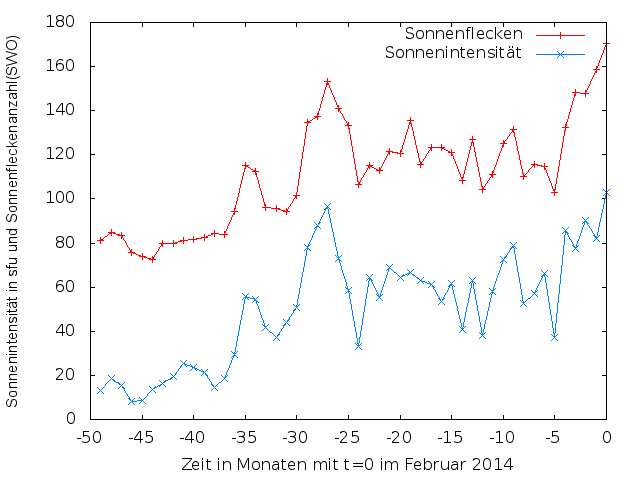
\includegraphics[width=.8\textwidth]{images/sunboth.png}
\caption{ Radiolichtkurve der Sonne und Anzahl der Sonnenflecken}
\label{fig:radioboth}
\end{figure}

Vergleicht man die Radiointensität mit den Sonnenflecken, stellt man fest, dass die Verläufe weitgehend übereinstimmen.